In this chapter, we will implement the GAN with two resNets algorithm on known true data distributions and try to visualize the evolution of data points and interpret the algorithm.\\
Let us first define the resNet that will be used in the following examples.
\begin{algorithm}
\caption{Forward Propagation Generator with $N_g$ as the number of layers}\label{alg:gen}
\textbf{Input: } $z \in \R ^{d}$ from prior input noise distribution\\
\textbf{Output: } $G(z) \in \R^{d}$ as generated point
\begin{algorithmic}
\State $dt \gets 0.1$
\State $X \gets z$
\For{$i \gets 1$ to $N_g$}
\State $X \gets X + dt * \Dense_{\tanh} (X; \theta_i^G) $
\EndFor
\State \Return $X$
\end{algorithmic}
$\Dense_{\tanh} : \R^{d} \times \Theta \mapsto \R^{d}$ is a simple neural layer, with $\tanh $ as the activation function and $\theta_i^G$ as parameters.
\end{algorithm}

\begin{algorithm}
\caption{Forward Propagation Discriminator with $N_d$ as the number of layers}\label{alg:disc}
\textbf{Input: } $x \in \R ^{d}$ \\
\textbf{Output: } $D(x) \in [0,1]$
\begin{algorithmic}
\State $dt \gets 0.1$
\State $X \gets x$
\For{$i \gets 1$ to $N_d$}
\State $X \gets X + dt * \Dense_{\tanh} (X; \theta_i^D) $
\EndFor
\State $X \gets \Dense_{\sigma} (X)$
\State \Return $X$
\end{algorithmic}
$\Dense_{\tanh} : \R^{d} \times \Theta \mapsto \R^{d}$ is a simple neural layer, with $\tanh $ as the activation function and $\theta_i^G$ as parameters. $\Dense_{\sigma}: \R^d \mapsto [0,1]$, defined as $Dense_{\sigma}(X) = \sigma(w^TX+b) $, is a fixed simple neural layer with the sigmoid activation function with parameters $w, b$.
\end{algorithm}

\begin{algorithm}
\caption{Minibatch stochastic gradient descent training of generative adversarial nets.}\label{alg:grad_d}
Denote $\theta_g = (\theta_1^G,...,\theta_{N_g}^G)$; $\theta_d = (\theta_1^D,...,\theta_{N_d}^D)$\\
\textbf{Parameters: } Learning rate of generator and discriminator: $\alpha_g, \alpha_d$
\begin{algorithmic}
\For {number of iteration steps}\do \\
\begin{itemize}
\item  Sample minibatch of m noise samples $\{z_1 , ..., z_m\}$ from prior input noise distribution $p_z$
\item  Sample minibatch of m true examples $\{x_1 , ..., x_m\}$ from true data distribution $p_x$
\end{itemize}
Update the discriminator by ascending its stochastic gradient:
\State $$\theta_g \gets \theta_g +\alpha_g \nabla_{\theta_g} \frac{1}{m}\sum_{i = 1}^{m}[\log D(x_i)+\log(1-D(G(z_i)))]$$\\
Update the generator by descending its stochastic gradient:
\State $$\theta_d \gets \theta_d -\alpha_d \nabla_{\theta_d} \frac{1}{m}\sum_{i = 1}^{m}[\log (1-D(G(z_i)))]$$
\EndFor
\end{algorithmic}
\end{algorithm}

\newpage
\section{Uniform Distribution Experiment}
We begin with learning the true distribution of a uniform $[0,1] \times [0,0.5]$ distribution and we fix the prior input noise distribution as a uniform $[0,1] \times [0.5,1]$ distribution, shown as the following figure.\\
\begin{figure}[h]
    \centering
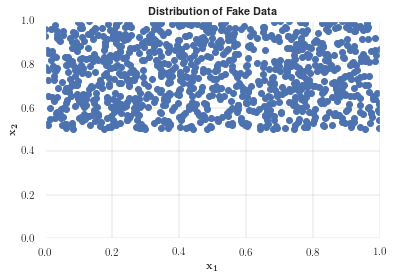
\includegraphics[width = 8cm]{Fake Uniform Distribution.png}
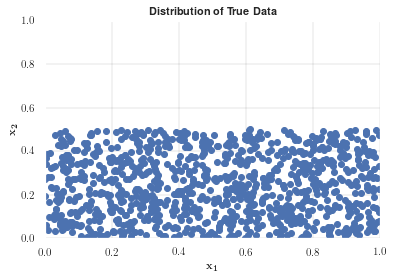
\includegraphics[width = 8cm]{True Uniform Distribution.png}
\caption{Distribution of true and fake data}
    \label{fig:uniform_distri}
\end{figure}
\subsection{Fix Generator; Train the Discriminator}
\label{sec: 1}
We first fix the generator and train the discriminator and after the training, we will try visualizing the process by feeding the discriminator points from both true and the fake distribution. The generator we choose is simply the identity one, meaning $G(z) = z$. The discriminator is a resNet according to Algorithm \ref{alg:disc} with $N_d=20$ layers. We set the learning rates at $\alpha_g = 0, \alpha_d = 0.001$. We use a mini-batch stochastic gradient descent with batch size $m = 100$ and 5000 iterations. Figure \ref{fig:gen_freeze_loss} shows the loss for both the generator and discriminator.
\begin{figure}[H]
    \centering
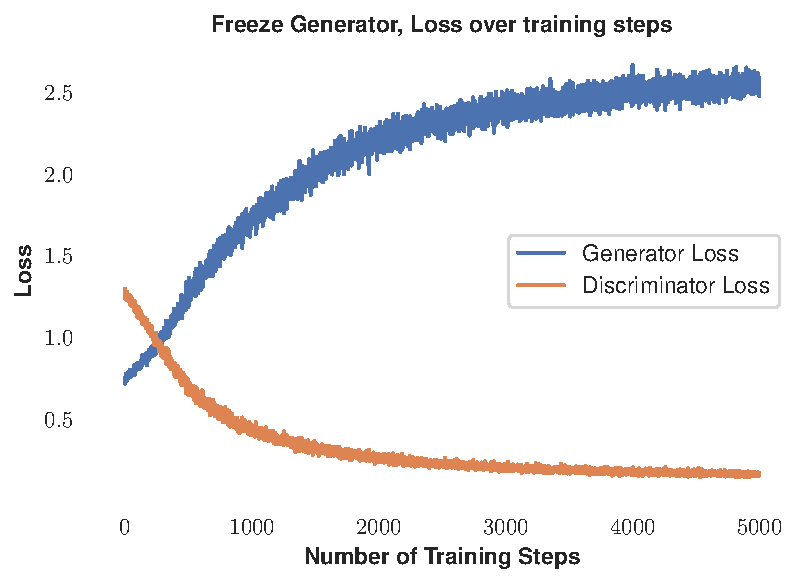
\includegraphics[width = 10cm]{Freeze_generator.pdf}
\caption{Loss over iteration}
    \label{fig:gen_freeze_loss}
\end{figure}
We observe that the discriminator loss decreases as generator loss increases, which is consistent to the fact that they are in a minimax game. The improvement of discriminator is at the cost of the higher generator loss. Although it is a simple training experiment, we can visualize the discriminator of how it discriminates data from true distribution and fake distribution through forward propagation, in other words, the evolution of points. Figure \ref{fig:evo_1} shows the evolution of true/fake data points in the process of the discriminator. The same plot also shows whether the capacity of the discriminator resNet is enough. Note that in the forward propagation algorithm, the maximum change in each coordinate of input $x$ is $\pm 0.1$ because the layer is activated by  $\tanh(x)\in (-1,1)$. Therefore in the two dimensional case with a 20-layer resNet, the maximum distance $x$ can move is $2\sqrt{2}$. We will see if the points can be moved in the correct regions within such distance.
\begin{figure}[H]
    \centering
    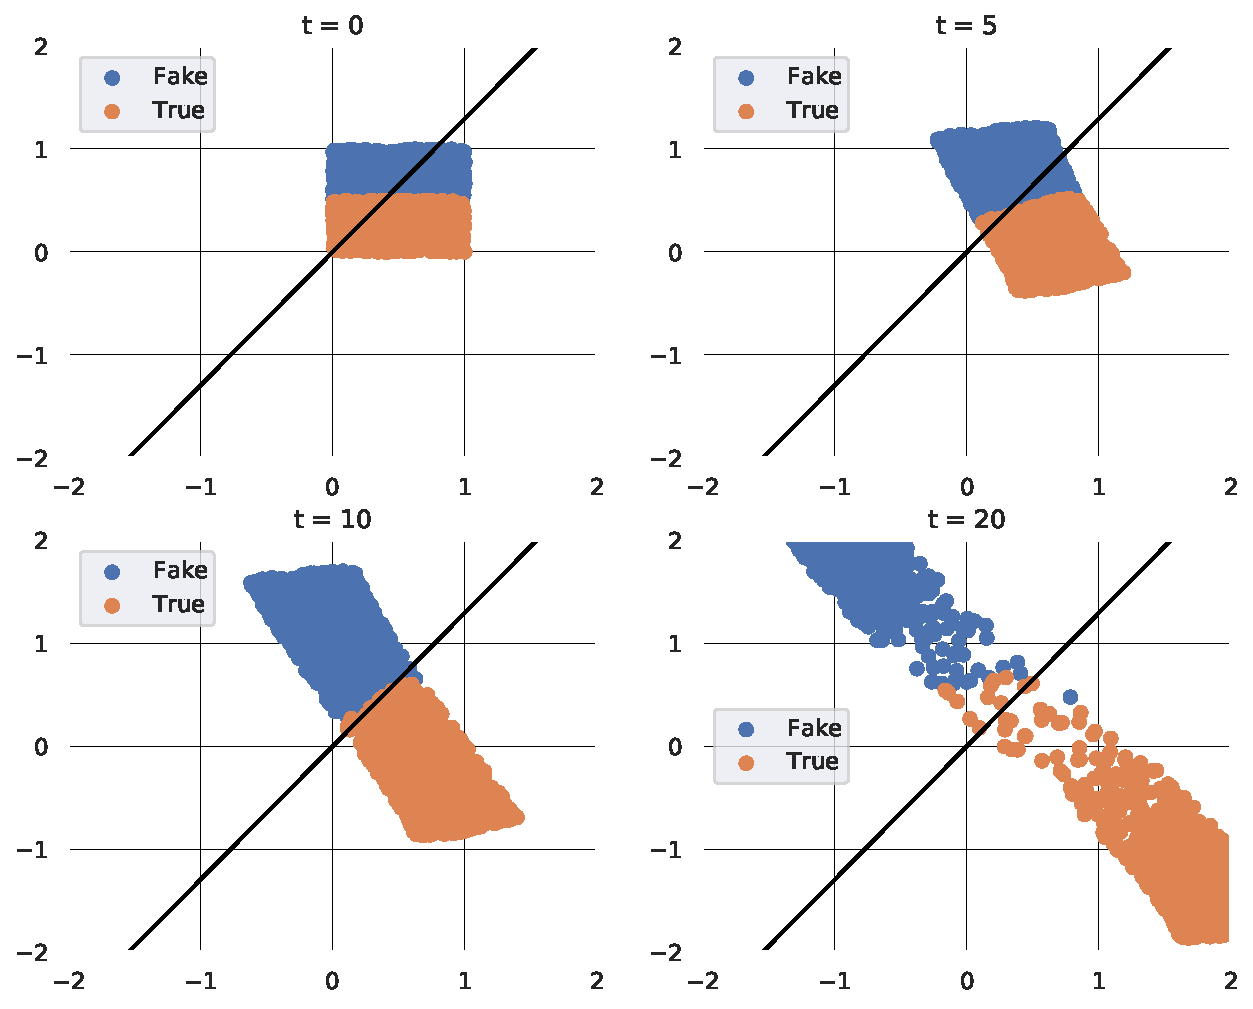
\includegraphics[width = 13cm]{Evo_1.pdf}
    \caption{Evolution of Points through Discriminator}
    \label{fig:evo_1}
\end{figure}
The black line is defined as $w^Tx +b =0$ according to the Algorithm \ref{alg:disc}, which is the decision boundary fixed by the last layer of the discriminator. We can see that as the process goes on, points are moved further away from the line accordingly. It shows how the control "drags" the points to their corresponding regions in order to minimize the terminal cost. Since moving distance of the points to the corresponding region is much less than $20\sqrt{2}$, we can determine that the discriminator resNet has enough capacity in this case.

\subsection{Fix Discriminator; Train Generator}
\label{sec: 2}
We now fix the discriminator with decision boundary $x_2 = 0.5$, meaning that points with $x_2 < 0.5$ will be classified as points from true distribution. We build the generator according to Algorithm \ref{alg:gen} with $N_g = 20$. We will use a learning rate $\alpha_g = 0.001, \alpha_d = 0$ and a mini-batch stochastic gradient descent with batch size $m = 100$ and 5000 iterations.
Figure \ref{fig:freeze_disc}, \ref{fig:distri_disc} shows the loss over the iteration steps and evolution of points under the control of generator.
\begin{figure}[H]
    \centering
    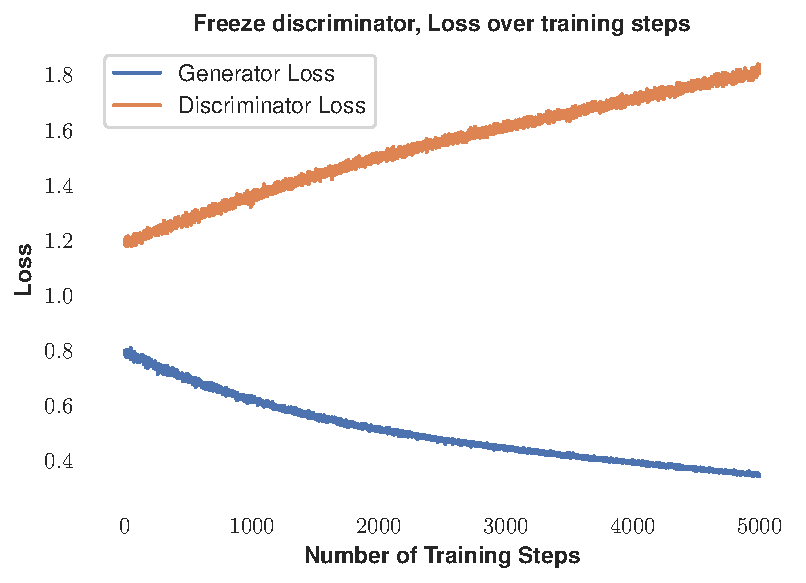
\includegraphics[width= 10cm]{Freeze_discriminater.pdf}
    \caption{Loss over iteration}
    \label{fig:freeze_disc}
\end{figure}
\begin{figure}[H]
    \centering
    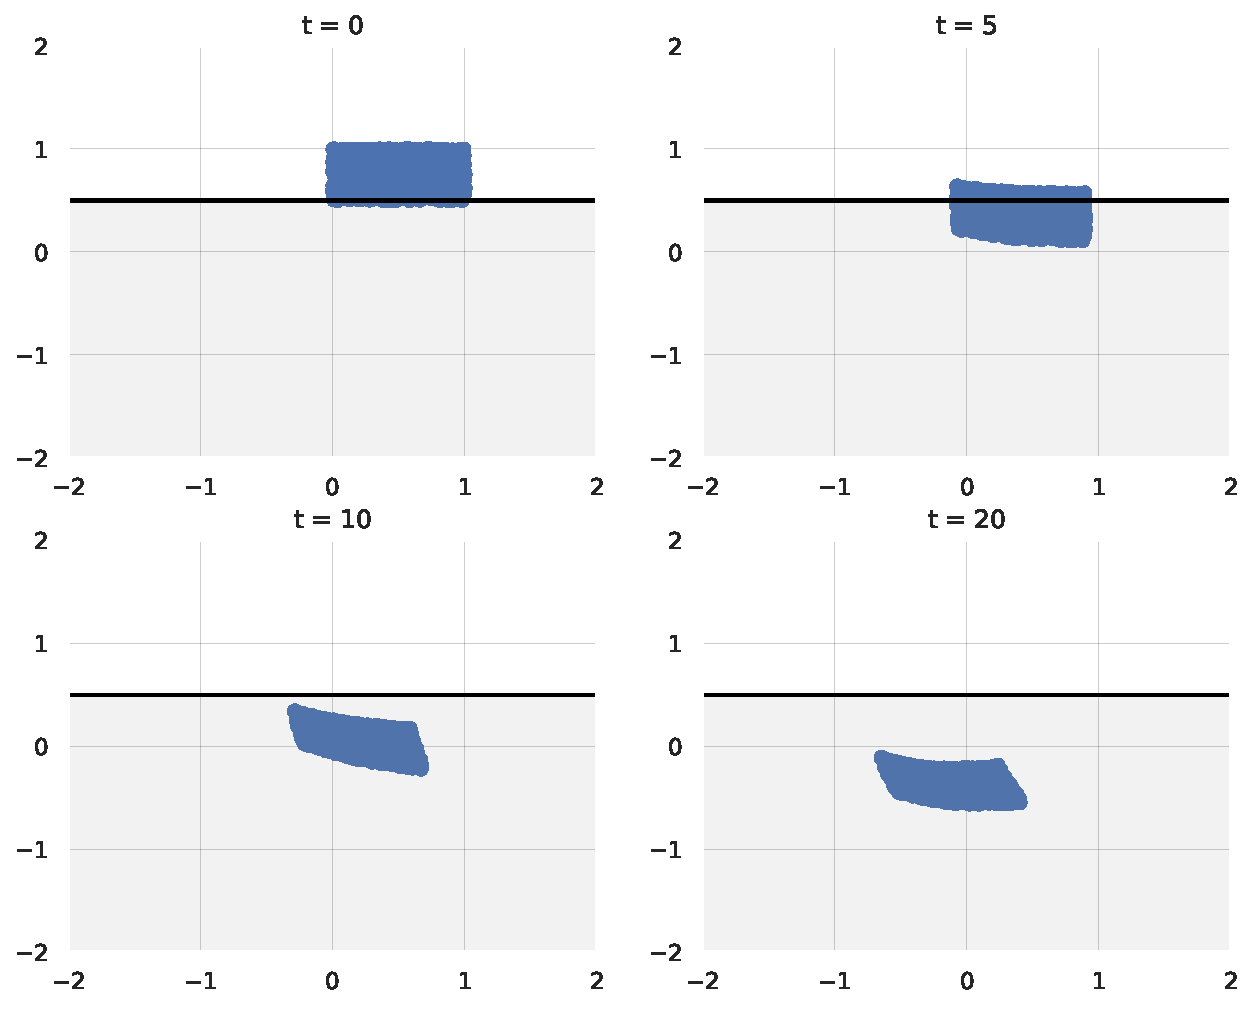
\includegraphics[width = 13cm]{Evo_2.pdf}
    \caption{Evolution of Points through Generator}
    \label{fig:distri_disc}
\end{figure}
Similarly, we can observe that the generator loss reduces at the cost of discriminator loss, illustrating the minimax game structure between the two. Moreover, in the evolution figure, the grey-shaded area is the target region and we can see the generator drags the points deeper and deeper into the target region to minimize the generator loss.
\subsection{GAN: Train the Generator and Discriminator at the same time}
Now, we have all the trivial cases done. Let's train the generator and discriminator together at the same time according to Algorithm \ref{alg:grad_d}. After training, we expect to have a good generator which can transform the noise inputs from the upper half (i.e. $[0,1] \times [0.5,1]$) to points from the true distribution, the lower half (i.e. $[0,1] \times [0,0.5]$). Moreover, in order to have a good generator, we must have a good discriminator beforehand to learn the rules of the true distribution and hence, "guide" the generator. In the experiment, I find the generator learns quicker than the discriminator with the learning rate pair $(\alpha_g,\alpha_d) = (0.001,0.001)$, meaning the minimax game is dominated by the generator. However, as the generator becomes too good before discriminator learns the features of true distribution, the algorithm requires more iterations to reach an equilibrium. In the following plots, I use $(\alpha_g,\alpha_d) = (0.0001,0.001)$. Additionally, comparing to trivial cases in the previous subsections, the real game dynamic between the generator and the discriminator complicates the training process and hence I use 10000 iterations. I will keep $N_g = N_d = 20$ the same as above because it has been validated that they have enough capacity. 
\begin{figure}[H]
    \centering
    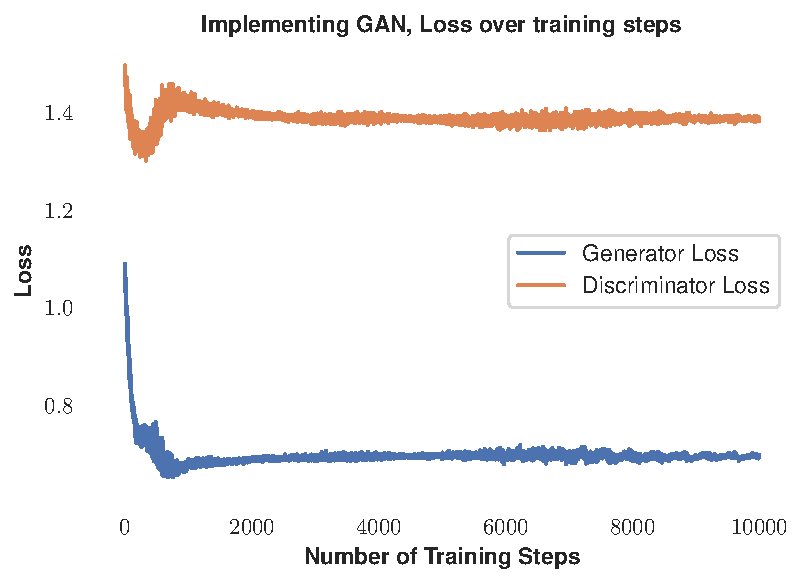
\includegraphics[width = 10cm]{GAN.pdf}
    \caption{Loss over iteration}
    \label{fig:Gan}
\end{figure}
\begin{figure}[H]
    \centering
    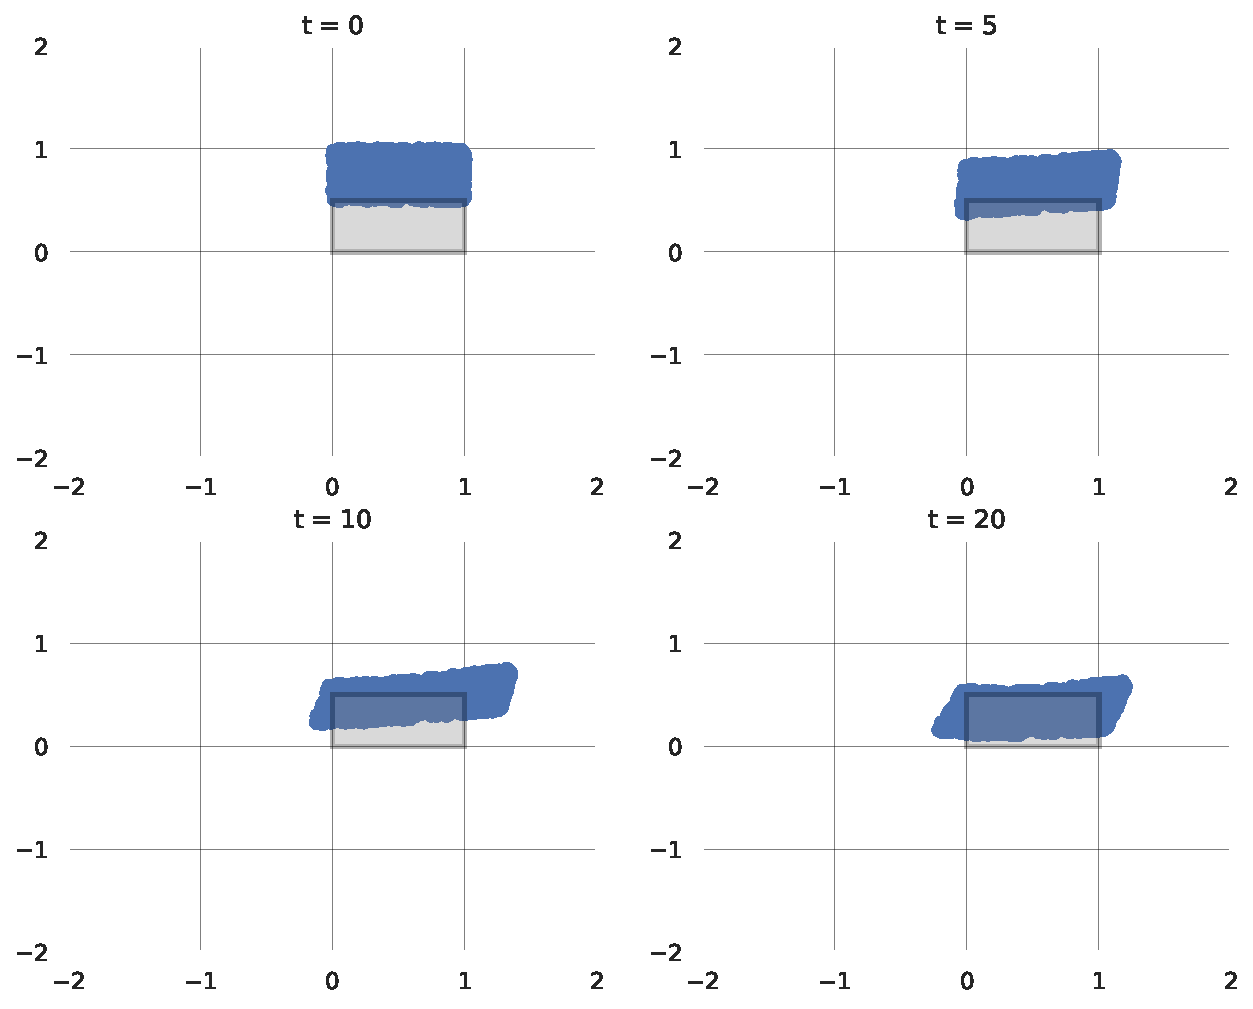
\includegraphics[width = 13cm]{Evo_3.pdf}
    \caption{Evolution of Points through Generator}
    \label{fig:GAN-gen}
\end{figure}
\begin{figure}[H]
    \centering
    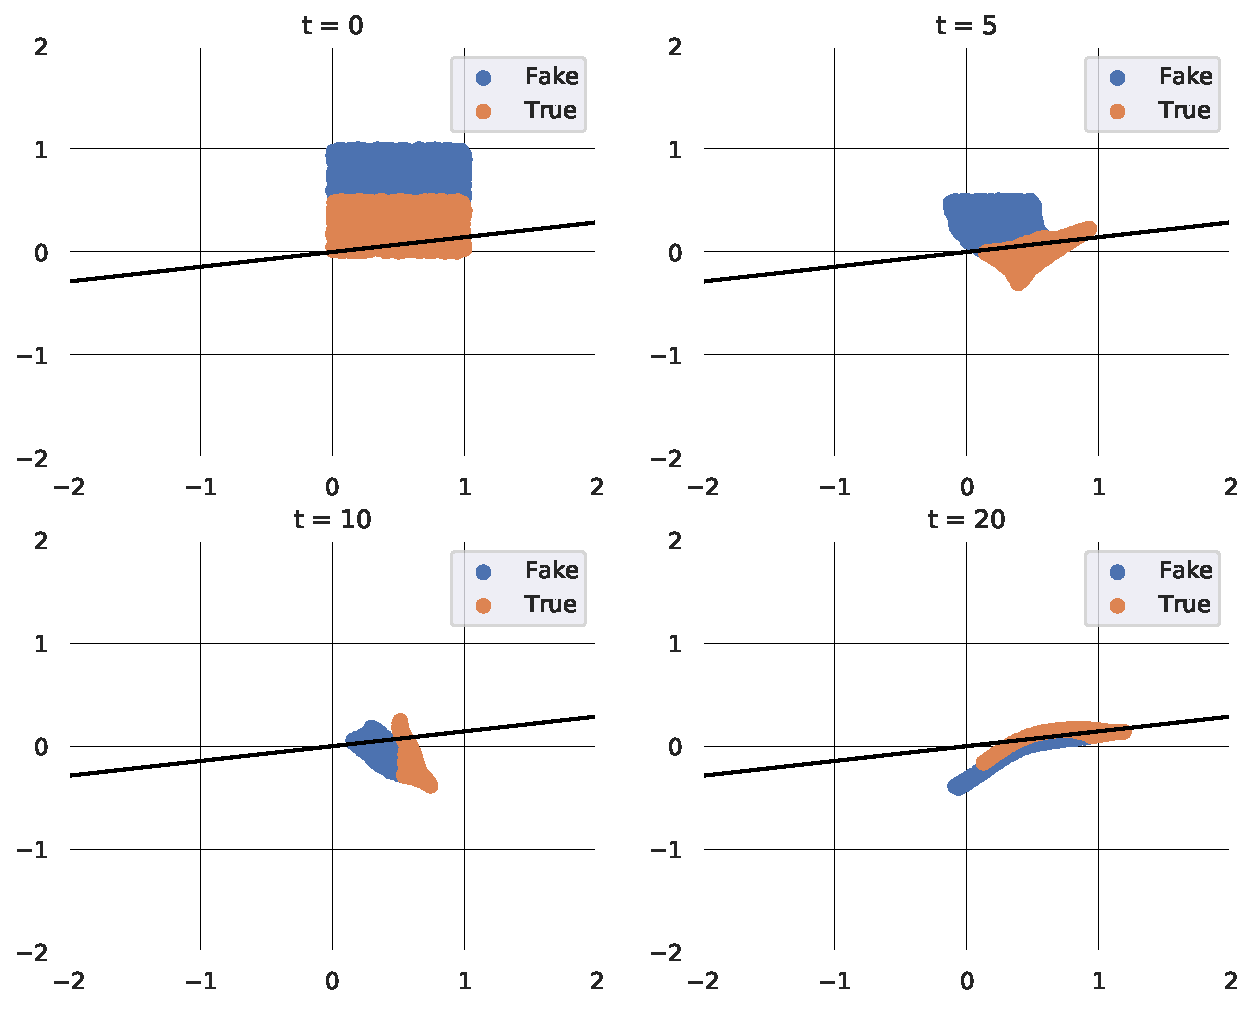
\includegraphics[width = 13cm]{Evo_4.pdf}
    \caption{Evolution of Points through Discriminator}
    \label{fig:GAN-disc}
\end{figure}
In Figure \ref{fig:GAN-gen}, the shaded area is the target region. We can see that a trained generator will move the points from the fake distribution in a way to imitate the true distribution in the end. However, we can see that some points are still out of the true distribution box. It means the generator is still not perfect after 10000 iterations and the two players have not reached a global optimality. In Figure \ref{fig:GAN-disc}, we observe that when $t = 20$, data points from both the true distribution and fake distribution clustered along the decision boundary. It illustrates that the generator is good enough to cheat the discriminator so that it is not able to decide whether the point is from the true distribution and fake distribution. Overall, we can conclude that given the discriminator, the generator is clever enough to cheat it while the discriminator has to learn more about the true distribution to guide the generator to a better result. In Figure \ref{fig:Gan}, because of the minimax game structure between the generator and the discriminator, it is difficult to visualize the improvement of the algorithm with only the plot of the loss over iterations. It is likely that the stable loss in later training steps means the algorithm is trapped in a local optimality while it can also mean both the generator and the discriminator are learning. We will provide more details in the next example.
\section{Normal Distribution Experiment}
In this section, we will conduct the same experiment on a different distribution: normal distribution. Let the true distribution be $(x_1,x_2)^T \sim \mathcal{N}\left((0,0)^T, \Sigma\right)$ and the fake distribution be $(z_1,z_2)^T \sim \mathcal{N}\left((1,1)^T, \Sigma\right)$, where $\Sigma = \begin{bmatrix}
0.05 & 0\\
0 & 0.05\\
\end{bmatrix}$. The discriminator is more difficult to train compared to the previous experiment because the data points from fake distribution and true distribution overlap. It means that even with a primitive generator (e.g. the identity), given a data point, the discriminator can not easily determine which distribution it comes from. 
\begin{figure}[H]
    \centering
    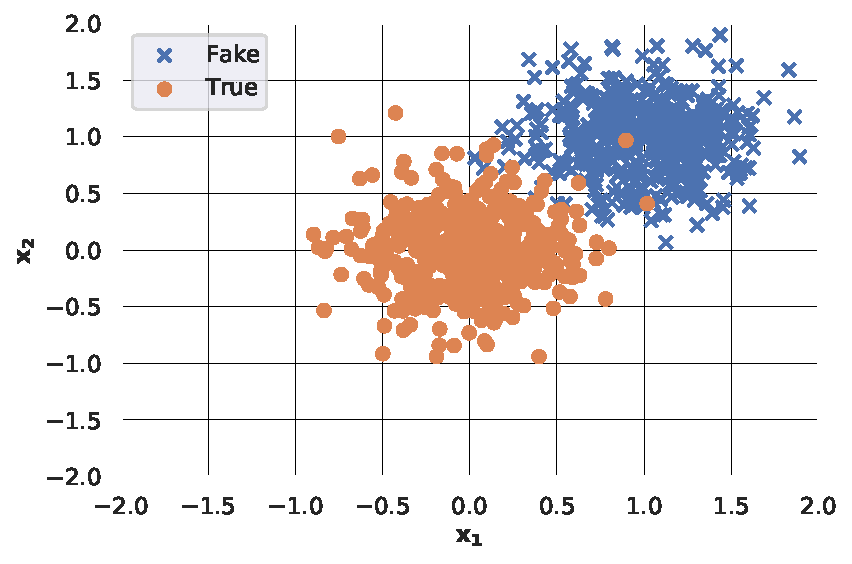
\includegraphics[width = 12cm]{Gaussian Distribution.pdf}
    \caption{Gaussian Distribution}
    \label{fig:gau}
\end{figure}
Figure \ref{fig:gau} shows samples from the true and fake distribution. In this experiment, we will omit the preliminary parts similar to section \ref{sec: 1}, \ref{sec: 2} and we directly train according to the \ref{alg:grad_d} algorithm.

As mentioned in the previous section, it is difficult to directly visualize the success of the algorithm by looking at the loss over iterations. Therefore, we will need a new measure of success. Since the true distribution is known, we will define the generated likelihood from a fixed noise input $z_1 , z_2 , ... , z_n$ as:
$$ \mathcal{L}(\theta^G) = \prod_{i = 1}^{n} f\left (G_{\theta^G}(z_i)\right), \text{   $f$ is the probability density function of true distribution}$$
In this case, 
$$ f (\boldsymbol{x}) =\frac{1}{\sqrt{(2 \pi)^{2} \cdot \det (\boldsymbol{\Sigma})}} e^{-\frac{1}{2}x^{T} 
\boldsymbol{\Sigma^{-1}} x},  \quad \Sigma \text{ is defined above}$$
We can further simplify in our case that to maximize the likelihood is equivalent to minimize the following $$l(\theta^G) = \sum_{i = 1}^{n} G(z_i)^T \Sigma^{-1} G(z_i) \propto \sum_{i = 1}^{n} ||G(z_i)||^2 ,$$
We will call this number the negative log-generated likelihood and we will use this to measure the success of the algorithm. Furthermore, to simplify, we will fix a group of test prior input noise points at the beginning and compute the number based on the points generated by those points. Ideally, we will see this number decrease which indicates that the probability that such group of generated points are sampled from the true distribution increases, meaning the generator is improving. Due to the computational cost, we will take $n= 10$ samples from noise input and compute the log-generated likelihood.
We apply the same logic to deduce the capacity of the generator: We find that in this case the distance points from fake distribution have to travel is $(1,1) \rightarrow (0,0) = \sqrt{2}$ and we a 20-layered resNet has the maximum capacity to move points for a distance of $2\sqrt{2}$. Hence the capacity of $N_g = 20$ is reasonable. Similar to the case in uniform distribution, when training the GAN, we implement the learning rate $\alpha_g = 0.0001, \alpha_d = 0.001$ to avoid the dominance of the generator. We will set $N_d = 20$ and run the iterative algorithm \ref{alg:grad_d} for 10000 times.
We can see from Figure \ref{fig:gauiter} that during the first 2000 iterations, the generator loss and discriminator loss changes significantly and accordingly, the log generated likelihood decreases. It means that our algorithm is working. Moreover, we observe that the discriminator loss decreases at the beginning at the cost of the generator loss. We prefer this structure instead of the other way around because without an accurate discriminator, the generator will definitely fail in imitating the true distribution. Also, it validates that our learning rate pair is wisely chosen. After about 2000 iterations, we find the losses are relatively stable and the log generated likelihood remains almost the same. It suggests that after 2000 training steps, the algorithm ceases to learn and is close to a local optimality. Figure \ref{fig:comparison} shows the result of generated distribution. We can see that the generated distribution and true distribution are very similar.
Figure \ref{fig:evo_dis_gau} shows how points from two distributions evolves under the control of the discriminator. It is worth noting that in this case, the discriminator outputs all the points centered along the decision boundary, indicating that the generator is well trained. Figure \ref{fig:evo_gen_gau} shows how points from noise prior distribution evolve under the control of the discriminator. 
\begin{figure}
    \centering
    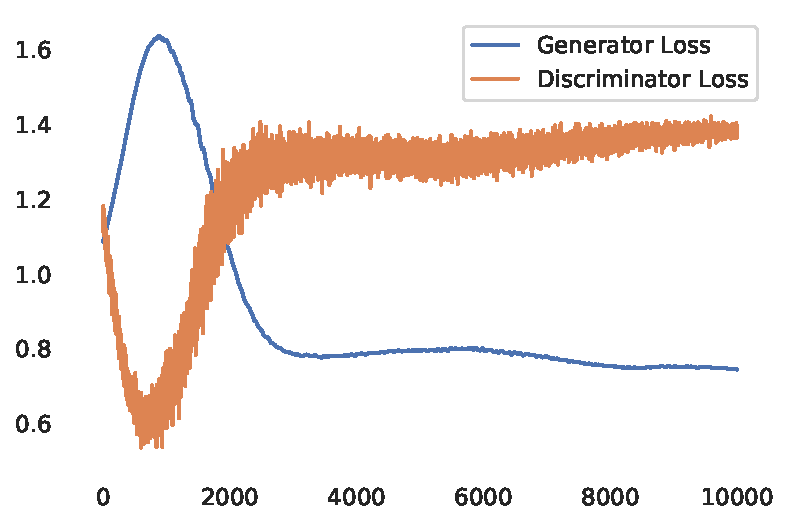
\includegraphics[width = 8cm]{GAN_gau.pdf}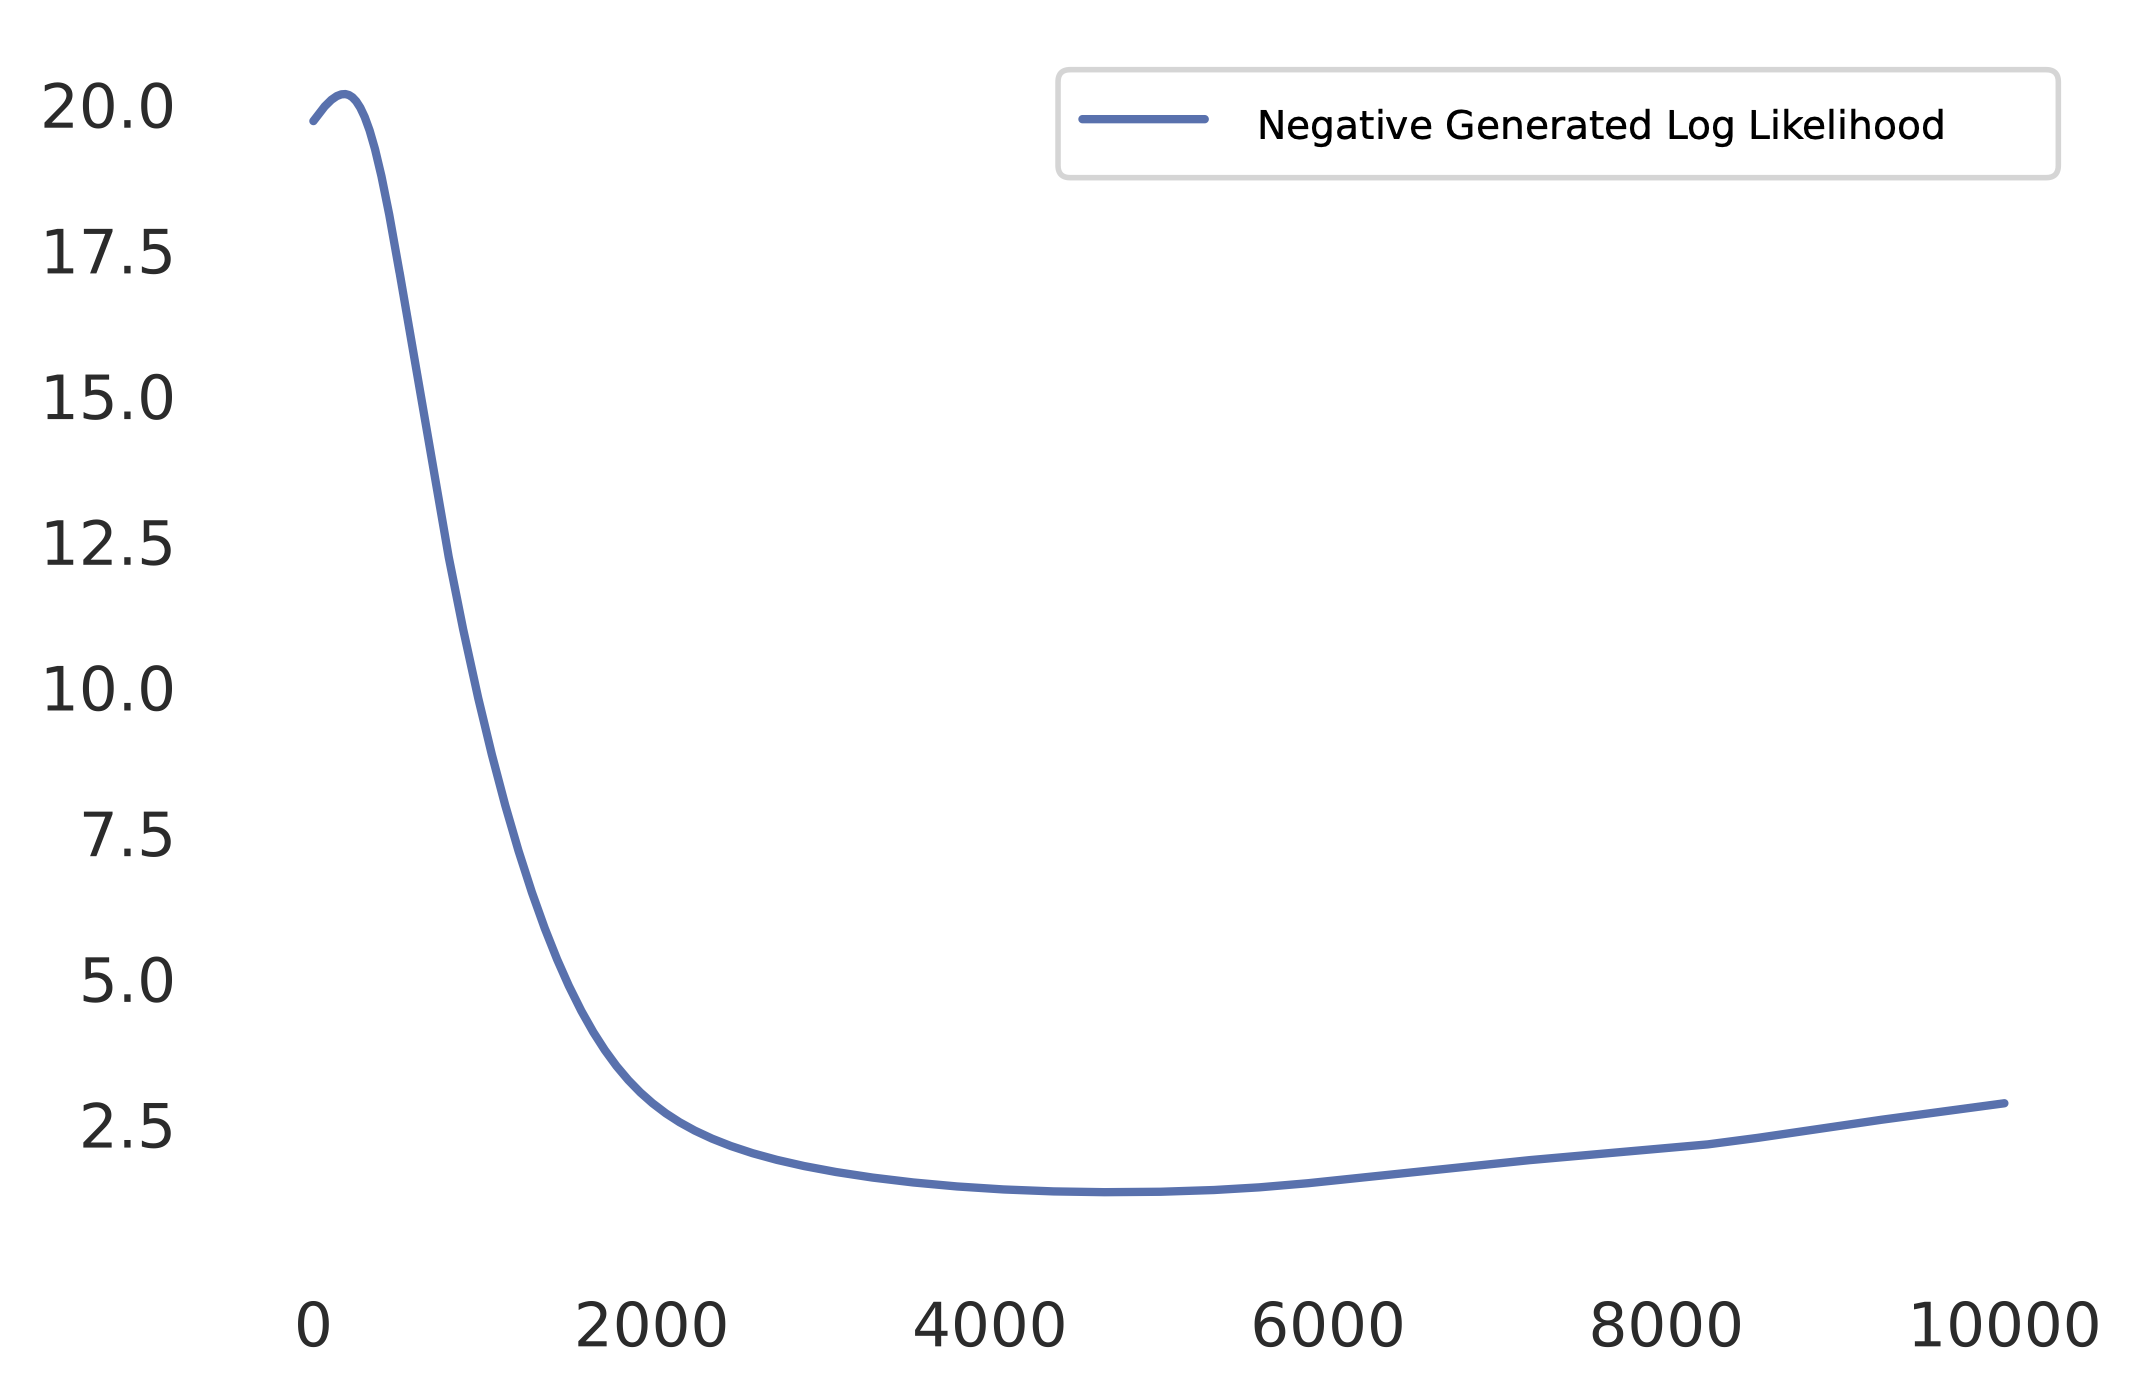
\includegraphics[width = 8cm]{GAN_gau_likeli.png}
    \caption{Loss, negative log-generated likelihood over iteration}
    \label{fig:gauiter}
\end{figure}
\begin{figure}
    \centering
    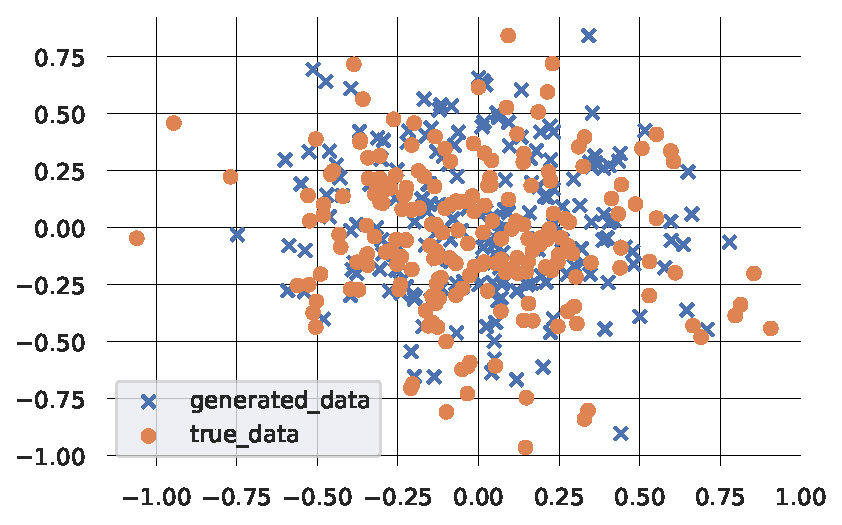
\includegraphics[width = 13cm]{comparison.pdf}
    \caption{Generated Data vs. True Data}
    \label{fig:comparison}
\end{figure}
\begin{figure}
    \centering
    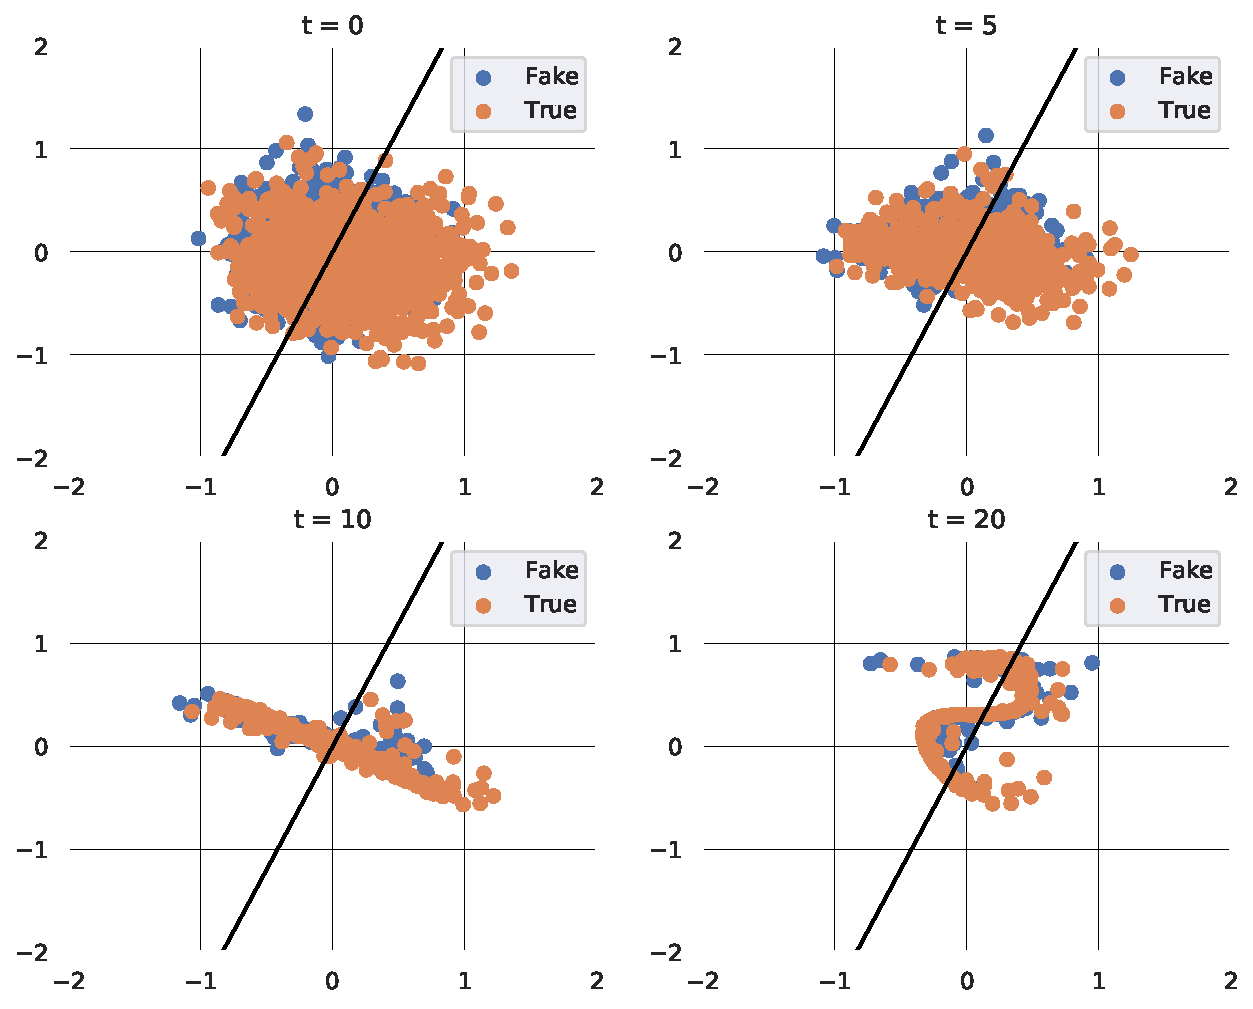
\includegraphics[width = 13 cm]{Evo_5.pdf}
    \caption{Evolution of Points through Discriminator}
    \label{fig:evo_dis_gau}
\end{figure}
\begin{figure}
    \centering
    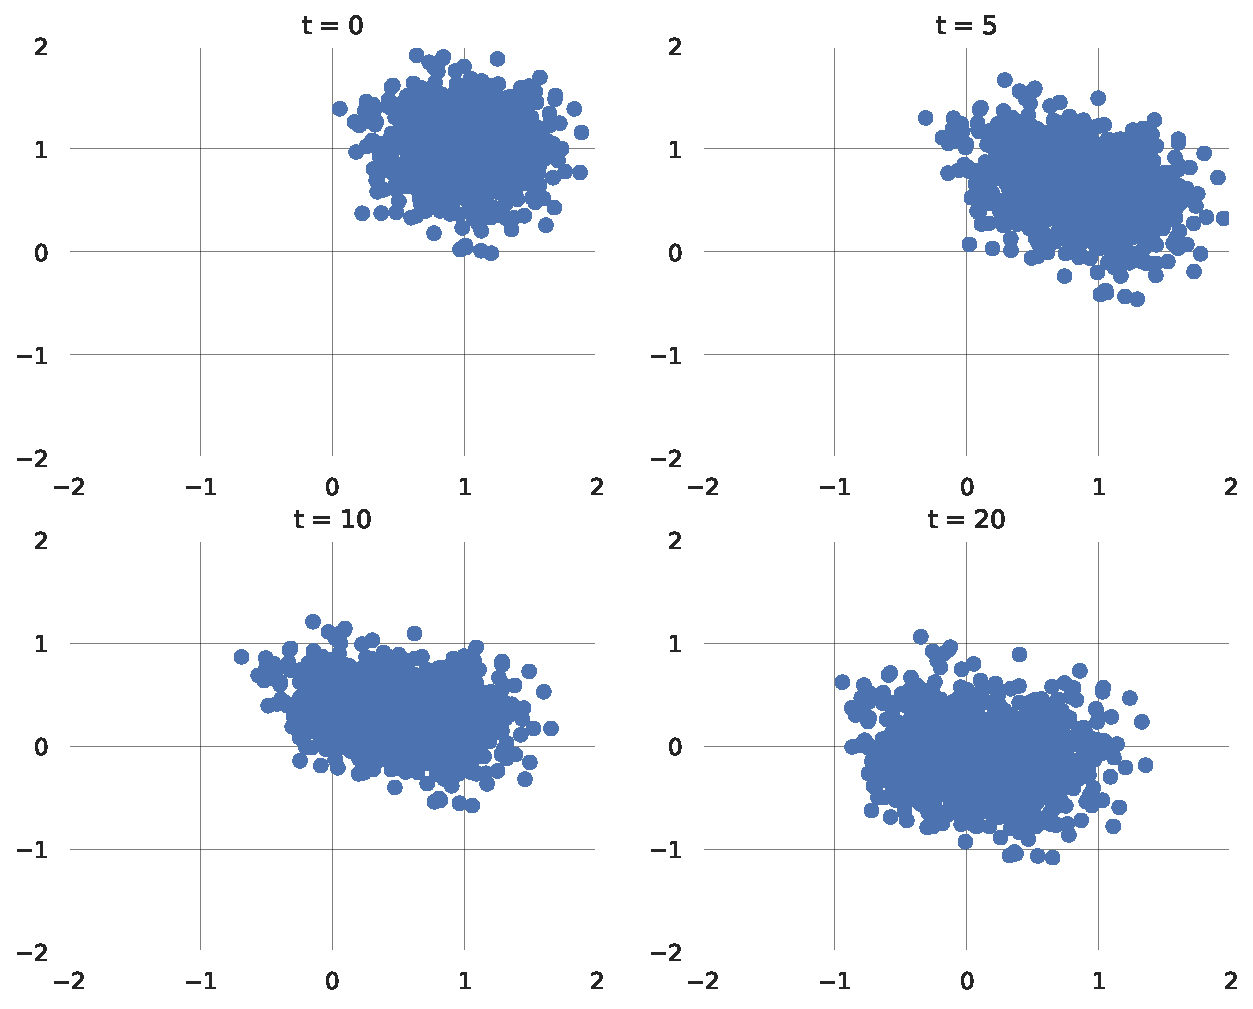
\includegraphics[width = 13 cm]{Evo_6.pdf}
    \caption{Evolution of Points through Generator}
    \label{fig:evo_gen_gau}
\end{figure}

